\section{Análisis de las propiedades de los estimadores}
A continuación, procederemos a graficar los sesgos, varianzas y errores cuadráticos medios de los estimadores en función de distintos valores de \textbf{b} en el rango $(0, 2)$.

\subsection{Sesgo}
Analizaremos el sesgo de los estimadores utilizando la siguiente definición:
$$Sesgo(\hat{b}) = \hat{b} - b$$

\begin{figure}[H]
	\centering
	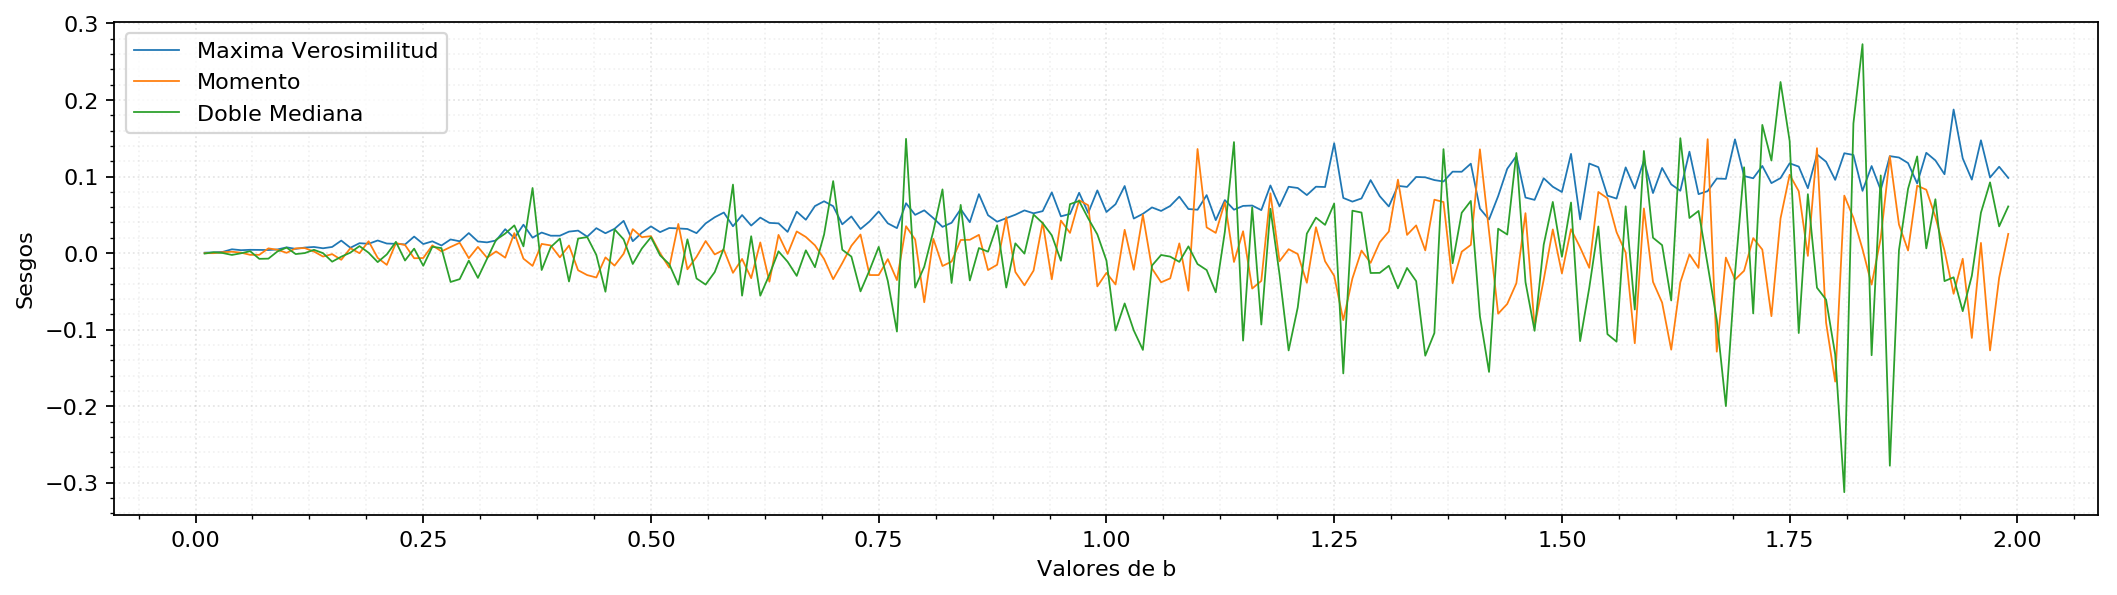
\includegraphics[width=1\textwidth]{imagenes/sesgos.png}
	\caption{\footnotesize Sesgos de los estimadores en función de los valores de \textbf{b}. $a=0, n=15$}
	\label{fig:ej6-sesgos}
\end{figure}

En la figura \ref{fig:ej6-sesgos} se puede observar que, a medida que el valor de $b$ aumenta, el valor absoluto del sesgo del estimador de $b$ también incrementa. Esto tiene sentido porque, por ejemplo, un error del 5\% en un estimador de $b=1$ sería $0,95$ o $1,05$, mientras que un error del 5\% en un estimador de $b = 100$ sería $95$ o $105$. Por eso, si bien la calidad del estimador no varía en función de $b$, sí lo hace la magnitud de sus sesgos. Grafiquemos la diferencia porcentual entre $\hat{b}$ y $b$ en función de $b$:

\begin{figure}[H]
	\centering
	\begin{minipage}[t]{.325\textwidth}
		\centering
		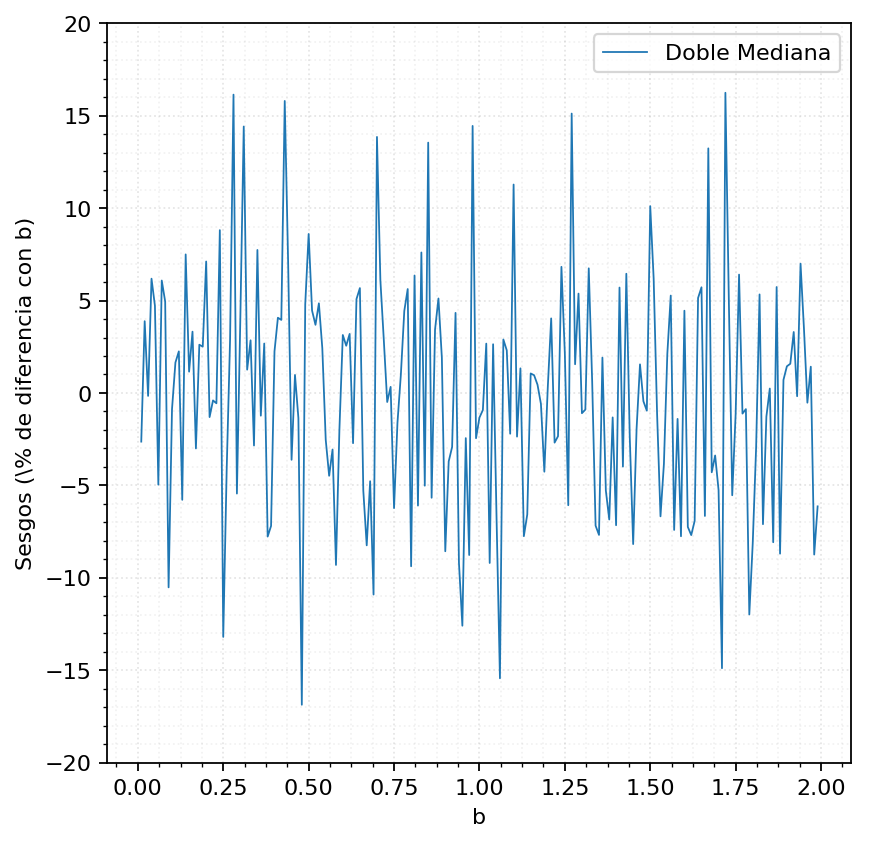
\includegraphics[scale=0.37]{imagenes/sesgos-med-porcentaje-err.png}
		\caption{\footnotesize Dif. \% entre $b$ y $\hat{b}_{med}$}
		\label{fig:ej6-sesgos-err-med}
	\end{minipage}
	\begin{minipage}[t]{.325\textwidth}
		\centering
		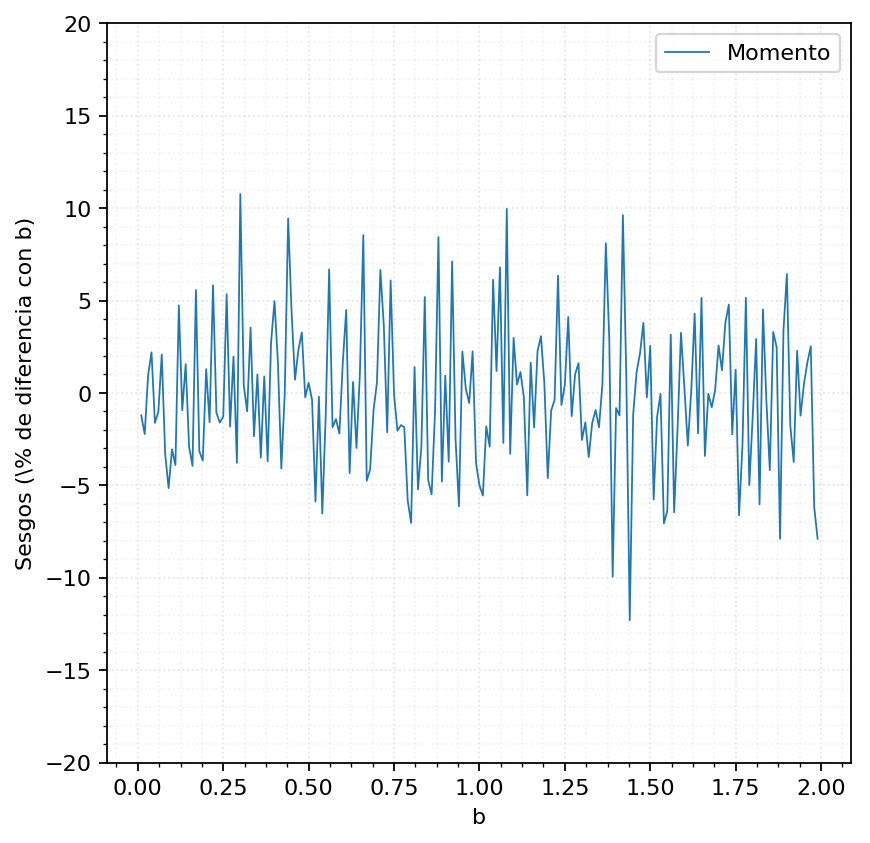
\includegraphics[scale=0.37]{imagenes/sesgos-mom-porcentaje-err.png}
		\caption{\footnotesize Dif. \% entre $b$ y $\hat{b}_{mom}$}
		\label{fig:ej6-sesgos-err-mom}
	\end{minipage}
	\begin{minipage}[t]{.325\textwidth}
		\centering
		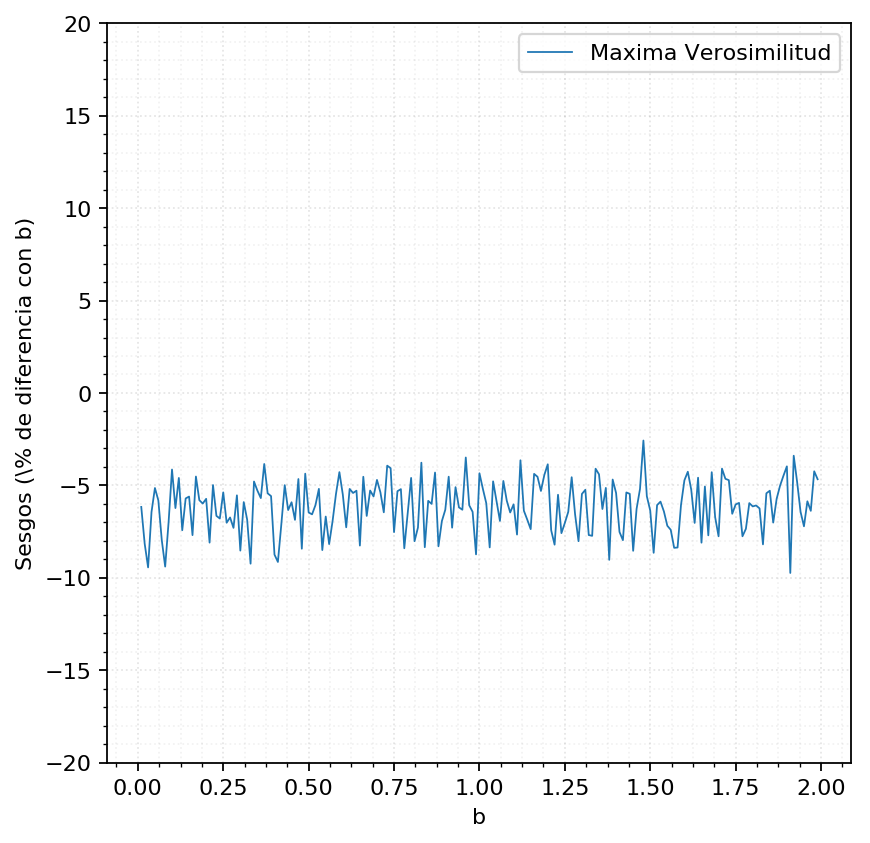
\includegraphics[scale=0.37]{imagenes/sesgos-mv-porcentaje-err.png}
		\caption{\footnotesize Dif. \% entre $b$ y $\hat{b}_{mv}$}
		\label{fig:ej6-sesgos-err-mv}
	\end{minipage}
\end{figure}

Podemos observar ahora que el porcentaje de diferencia entre $b$ y cada $\hat{b}$ tiene un comportamiento con cierta aleatoriedad pero siempre dentro de una cota, que tenderá a un módulo $0$ si el estimador respectivo es asintóticamente insesgado.

\vskip 8pt

También podemos ver que para el estimador $\hat{b}_{med}$, su diferencia porcentual con $b$ está entre el $-15\%$ y el $15\%$. La diferencia porcentual para el estimador $\hat{b}_{mom}$ está entre el $-10\%$ y el $10\%$ mientras que la diferencia porcentual para el estimador $\hat{b}_{mv}$ está entre el $-10\%$ y el $-5\%$. Esta cota está contenida en los números negativos debido a la naturaleza del estimador de máxima verosimilitud, que estima el valor de $b$ como el elemento de valor máximo dentro de la muestra analizada. Como la muestra en cuestión tiene distribución uniforme de parámetros $[0, b]$, un experimento uniforme jamás producirá un resultado mayor a $b$, por lo tanto el valor máximo de $\hat{b}_{mv}$ es $b$. Luego, el $sesgo(\hat{b}_{mv}) \leq 0$.

\subsubsection{Estimador de Máxima Verosimilitud}
Veamos si el estimador $\hat{b}_{mv}$ es asintóticamente insesgado. Para que lo sea, debemos ver que $E(\hat{b}_{mv}) = b$.
\begin{align*}
	E(\hat{b}_{mv}) = b &\iff \\
	E(max\{x_1, \dots, x_n\}) = b
\end{align*}
Para esto, debemos encontrar la función de densidad de la variable aleatoria $max\{x_1, \dots, x_n\}$:
\begin{align*}
	Y = max\{x_1, \dots, x_n\} \implies P(Y \leq y) &= \Big( P(X \leq y) \Big)^n = F_{Y}(y)
\end{align*}
Sabiendo que $X~U[0, b]$:
\begin{align*}
	F_{Y}(y) = 
	\begin{cases}
		0 						&\mbox{si } n y \leq 0 \\
		\Big(\frac{y}{b}\Big)^n & \mbox{si } 0 < y < b \\
		1 						& \mbox{si } y \geq b
	\end{cases}
\end{align*}
Luego, podemos derivar la función acumulada y obtener la función de densidad de $\hat{b}_{mv}$:
\begin{align*}
	f_{Y}(y) = \frac{n}{b} \cdot \Big(\frac{y}{b}\Big)^{n - 1} I_{(0, b)}(y)
\end{align*}
Ahora podemos calcular la esperanza del estimador:
\begin{align*}
	E(\hat{b}_{mv}) = E(Y) 	&= \int_{0}^{b}y \cdot \frac{n}{b} \cdot \Big(\frac{y}{b}\Big)^{n - 1} \\
							&= (\frac{n}{n+1}) \cdot b \neq b
\end{align*}
Por lo tanto, podemos concluir que el estimador de máxima verosimilitud \textbf{no es insesgado}. Sin embargo, el estimador \textbf{sí es asintóticamente insesgado} porque su límite tiende al parámetro $b$ cuando $n \rightarrow \infty$.

\subsubsection{Estimador de Momentos}
Averiguemos si el estimador de momentos es insesgado o asintóticamente insesgado:
\begin{align*}
	E(\hat{b}_{mom}) &= E(2\bar{X}) \\
	 	 			 &= 2 \cdot E(\frac{\sum_{i=1}^{n}X_{i}}{n}) \\
	 	 			 &= 2 \cdot \Big(\frac{1}{n}\Big) \cdot n \cdot E(x_{i}) \text{ (por indep.)}\\
	 	 			 &= 2 \cdot b \neq b
\end{align*}
Por lo tanto, el estimador de momentos no es insesgado. Tampoco es asintóticamente insesgado porque:
\begin{displaymath}
\lim_{n \to \infty} 2 \cdot b = 2 \cdot b \neq b
\end{displaymath}

\subsubsection{Estimador de la Doble Mediana}
Averigüemos si el estimador de la doble mediana es insesgado o asintóticamente insesgado:
\begin{align*}
	E(\hat{b}_{med}) &= E(2\tilde{X}) \\
	 	 			 &= 2 \cdot E(\tilde{X}) \\
	 	 			 &= 2 \cdot \Big(\frac{b - a}{2}\Big) \text{ (por indep. y L.G.N.)}\\
	 	 			 &= 2 \cdot \Big(\frac{b}{2}\Big) \\
	 	 			 &= b
\end{align*}
Por lo tanto, el estimador de la doble mediana es insesgado. Esto implica que también es asintóticamente insesgado.

\subsection{Varianza}
\begin{figure}[H]
	\centering
	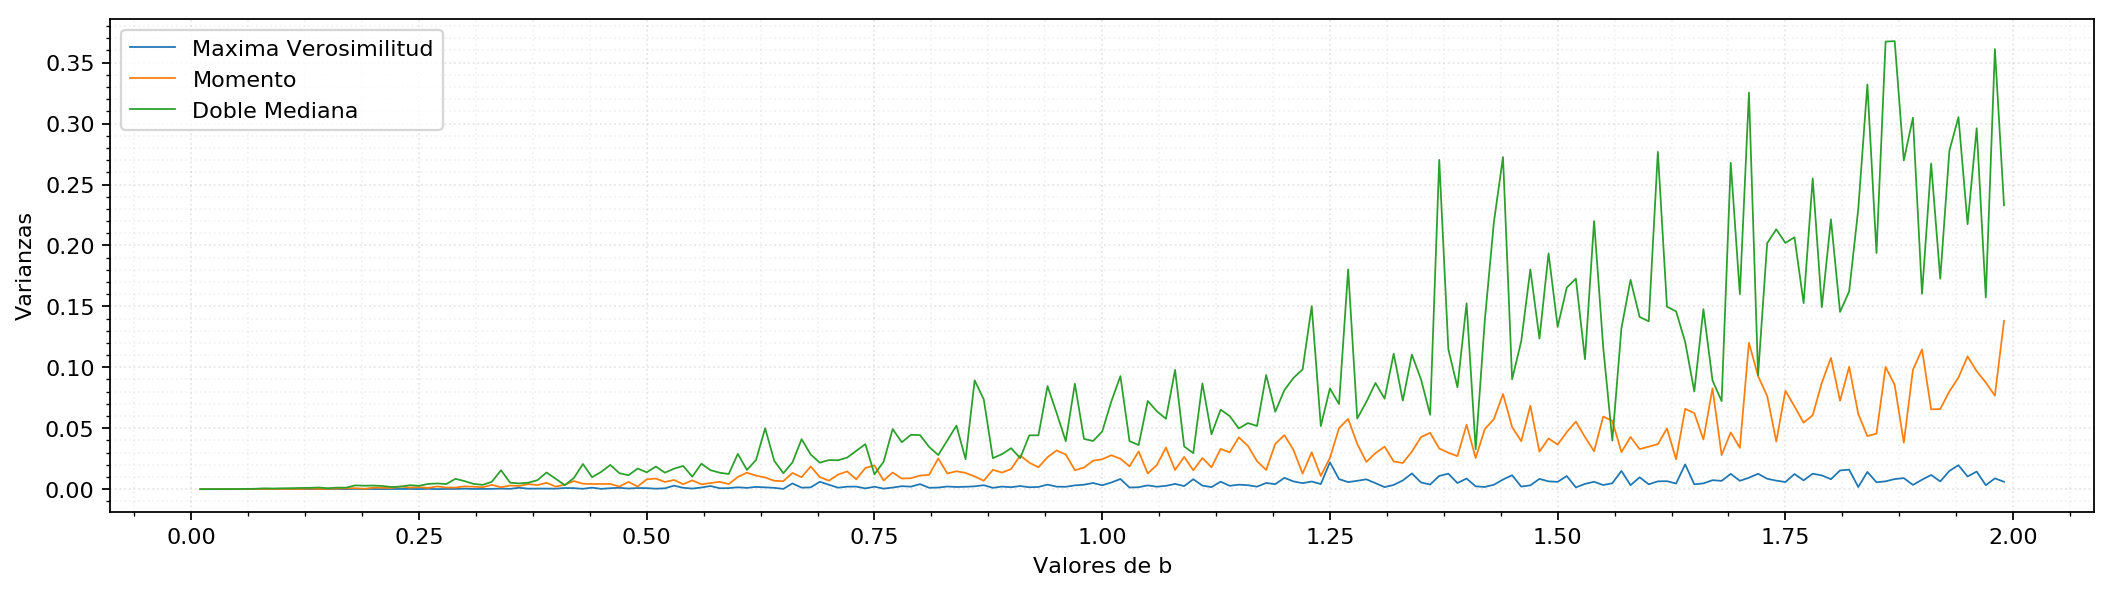
\includegraphics[width=1\textwidth]{imagenes/varianzas.png}
	\caption{\footnotesize Varianzas de los estimadores en función de los valores de \textbf{b}. $a=0, n=15$}
	\label{fig:ej6-varianzas}
\end{figure}

La figura \ref{fig:ej6-varianzas} nos muestra el comportamiento de las varianzas. Podemos observar que la varianza del estimador de la doble mediana $\hat{b}_{med}$ tiene el mayor crecimiento al variar $b$, seguida por la varianza del estimador $\hat{b}_{mom}$ y en último lugar, la varianza del estimador $\hat{b}_{mv}$.

% \subsubsection{Varianza del Estimador de Doble Mediana}
% \begin{align*}
% 	V(\hat{b}_{med}) &= E(\hat{b}^{2}_{med}) - \Big(E(\hat{b}_{med})\Big)^2 		\\
% 					 &= E(2 \ \cdot \tilde{X}^2) - \Big(E(2 \ \cdot \tilde{X})\Big)^2 \\
% 					 &= 4 \cdot \Bigg( E(\tilde{X}^2) - \Big(E(\tilde{X}^2)\Big)^2\Bigg)	\\
% 	 	 			 &= 4 \cdot \Bigg( \Big(\frac{b}{2}\Big)^2 - \Big(\frac{b}{2}\Big)^2 \Bigg) \text{ (por indep.)}		\\
% 	 	 			 &= 4 \cdot 0 = 0
% \end{align*}
% Luego, la varianza del estimador $\hat{b}_{med}$ es cero.

\subsection{Error Cuadrático Medio}
\begin{figure}[H]
	\centering
	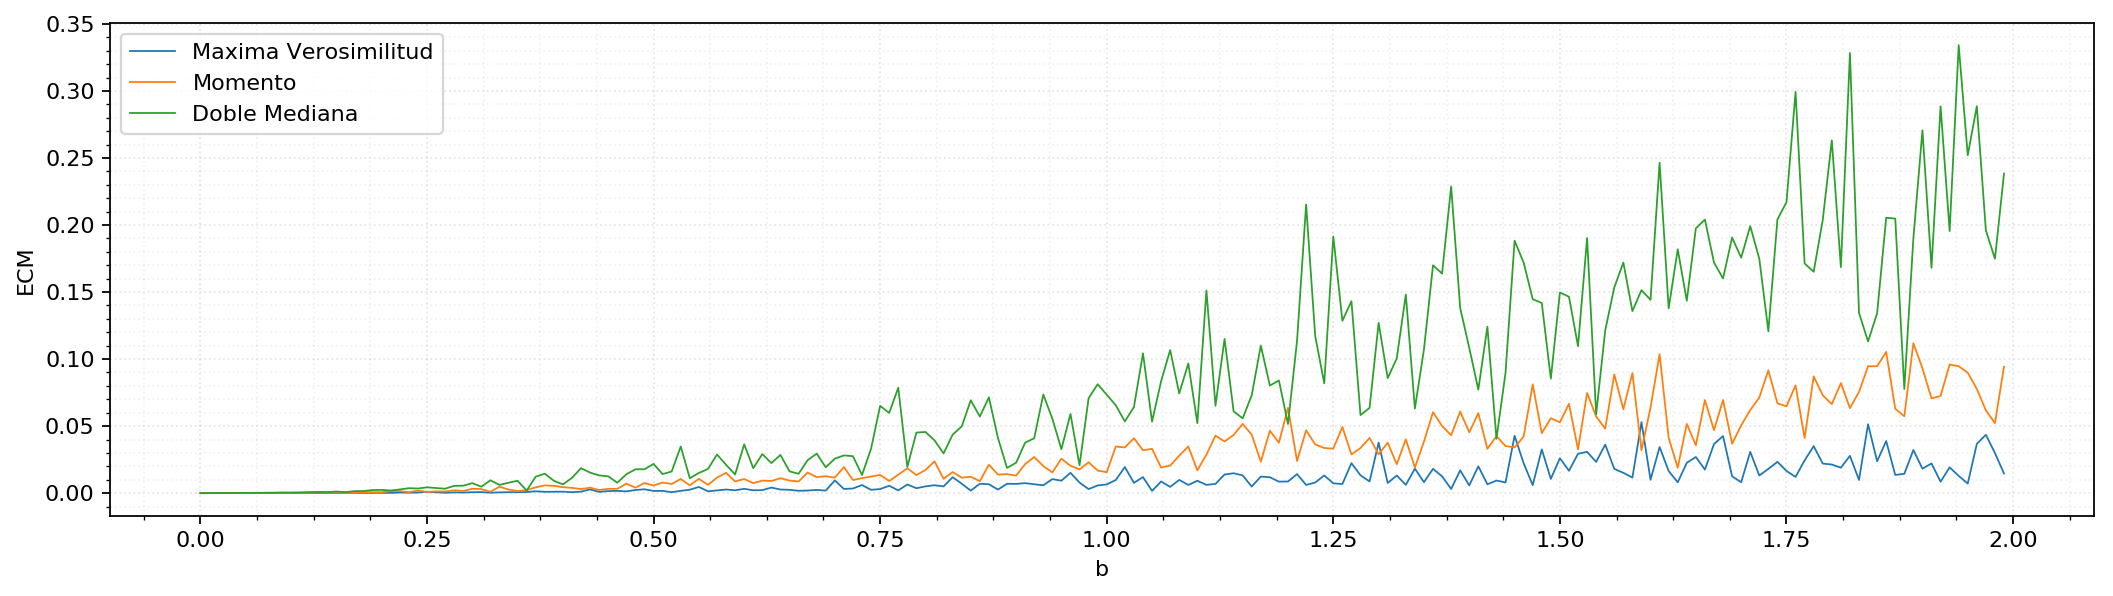
\includegraphics[width=1\textwidth]{imagenes/ecm.png}
	\caption{\footnotesize ECM de los estimadores en función de los valores de \textbf{b}. $a=0, n=15$}
	\label{fig:ej6-ecm}
\end{figure}

La figura \ref{fig:ej6-ecm} exhibe la tendencia del \textbf{Error Cuadrático Medio} a aumentar cuando el valor de $b$ lo hace también. Si bien el estimador $\hat{b}_{med}$ parece tender al mayor error cuadrático medio, es el único estimador insesgado y por lo tanto la mejor opción de entre los tres, dada una muestra de muchos elementos.